\documentclass[12pt,a4paper,titlepage]{memoir}
\usepackage[IS]{rubook}
\usepackage{ruthesis}

\title{M.Sc. (and BSc.) Thesis Template for \theInstitution{}}
\titleIS{M.Sc. (and B.Sc.) Thesis Template for \theInstitution{} in Icelandic}
\author{Joseph T. Foley}%Use \and as an author separator
\date{February 2020}% Change this to the date that it is signed
\dateIS{**Dagsetning í íslensk**}% Put the date in Icelandic

%\DocumentInfo{TYPE}{ABBREVIATION}{DEGREE}{PROGRAM}
%\DocumentInfo{Dissertation}{Ph.D.}{Doctor of Philosophy}{Computer Science}
\DocumentInfo{Dissertation}{Ph.D.}{Doctor of Philosophy}{Computer Science}
\School{School of Technology}

%% PhD only have Thesis Committee with roles.  Examiner is part of committee.
\SupervisorHeading{Thesis Committee}
\Supervisors{
  \personinfo{Superior A. Teacher}{Supervisor}{Professor}{Reykjavik University}{Iceland}
  \personinfo{Helpful A. Teacher}{Co-advisor}{Assistant Professor}{University of Iceland}{Iceland}
  \personinfo{Tough E. Questions}{Examiner}{Associate Professor}{Massachusetts Institute of Technology}{USA}
}

%%%%%% Useful Packages %%%%%%%%%%%%%%%%%%%%%%%%%%%%%%%%
\usepackage{lipsum}%provides us with text for testing
%% usage: \lipsum[STARTNUM-ENDNUM]

\usepackage[final]{listings}
%%% Formatting code inclusion and snippets
%% "final" option to force it to display code

%%%%%%%%%%%%%%%%%%%%%%%%%%%%%%%%%%%%%%%%%%%%%%%%%%%%%%%

\begin{document}

\maketitle
\copyrightpage{}
\signaturepage{}
\archivesigpage{}

\begin{abstract}
  The abstract goes here translated into English.
  If the thesis is in English, it should come first.
  It should be a fairly short summary of the entire document.
\end{abstract}

\begin{abstractIS}
  The abstract goes here translated into Icelandic.
  If the thesis is in Icelandic, it should come first.
  It should be a fairly short summary of the entire document.
\end{abstractIS}

\begin{dedications}
  I dedicate this to my spouse/child/pet/power animal.
\end{dedications}

\enableindents{}% turn on/off paragraph indents
% RUM: "Acknowledgements (optional)"%start numbering

\chapter*{Acknowledgements} 
\begin{quotation}
So long, and thanks for all the fish.
\end{quotation}\sourceatright{Douglas Adams\cite{adams84fish}}
\vspace{\baselineskip}

This work was funded by \the\year~RANNIS grant ``Survey of man-eating Minke whales'' 1415550.
Additional equipment was generously donated by the Icelandic Tourism Board.

{\em Acknowledgements are optional; comment this chapter out if they are absent
  Note that it is important to acknowledge any funding that helped in the work}

\clearpage{}
\tableofcontents{}\clearpage
\listoffigures{}\clearpage
\listoftables{}\clearpage

%% The list of abbreviations is an example of a special list
%% Other lists may be added, such as lists of algorithms, symbols, theorems, etc.
%% IN CS PhD, this is sometimes centered.
\chapter*{List of Abbreviations}%%RUM: Not mentioned
\begin{tabular}{ll}
M.Sc. &Masters of Science\\
Ph.D. &Doctor of Philosophy\\
\end{tabular}

\chapter*{List of Symbols}%%RUM: Not mentioned
\begin{tabular}{lll}
Symbol &Description &Value/Units\\
$E$ &Energy &\si{\joule}\\
$m$ &Mass &\si{gram}\\
$c$ &Speed of Light &\SI{2.99E8}{\meter\per\second\square}\\
\end{tabular}


\mainmatter{}
\aliaspagestyle{chapter}{empty}
% Don't put page numbers on the chapter changes

%% If you would like to separate chapters into different files, use
%% \include{chapterfile}
%% WARNING: Make sure that all of these files (and any new ones)
%% are UTF-8 otherwise you will get weird encoding errors.
\part{The First Part} % Parts optional but useful in longer documents
\chapter{The First Chapter}
\chapter{Introduction\label{cha:introduction}}
%% \ifdraft only shows the text in the first argument if you are in draft mode.
%% These directions will disappear in other modes.
State the objectives of the exercise. Ask yourself:
\underline{Why} did I design/create the item? What did I aim to
achieve? What is the problem I am trying to solve?  How is my
solution interesting or novel?

\section{Background}
Provide background about the subject matter (e.g. How was morse code
developed?  How is it used today?.

This is a place where there are usually many citations.
It is suspicious when there is not.
Include the purpose of the different equipment and your design intent. 
Include references to relevant scientific/technical work and books.
What other examples of similar designs exist?
How is your approach distinctive?

If you have specifications or related standards, these must be
described and cited also.  As an example, you might cite the specific
RoboSub competition website (and documents) if working on the lighting system for an AUV\cite{guls2016auvlight}\index{AUV}

\section{Example Section}
\begin{figure}
  \centering
  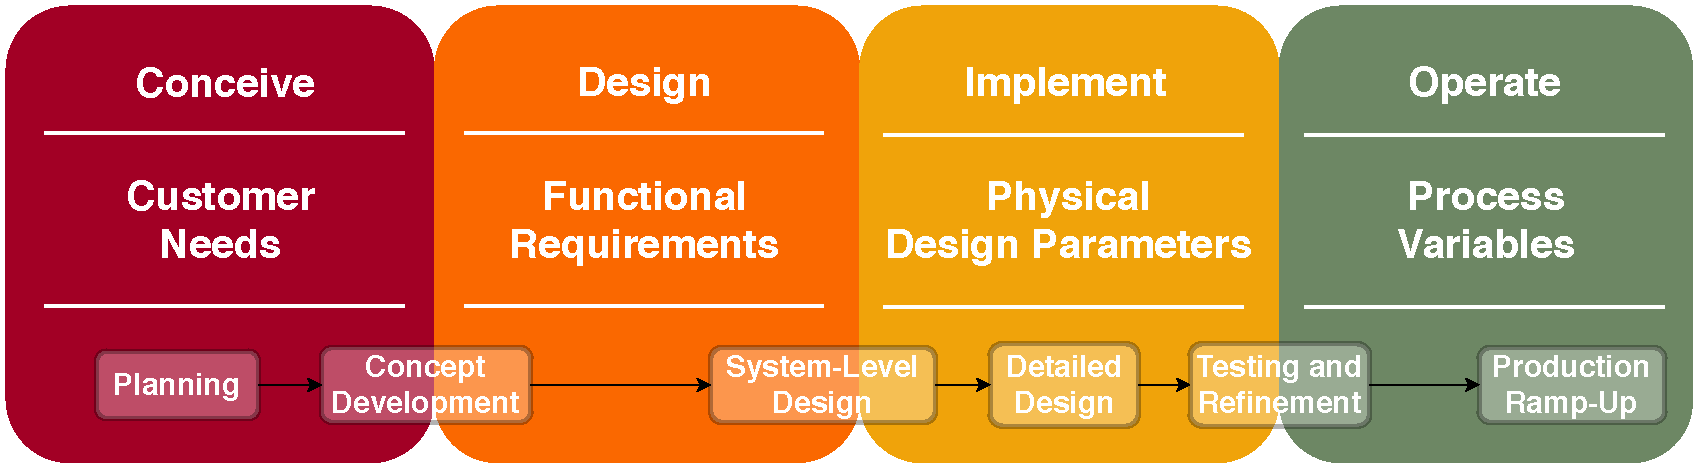
\includegraphics[width=0.8\textwidth]{design-commonalities}
  \caption[Design]{Design Commonalities\cite{foley2021dindesign}}\label{fig:ru-logo}
\end{figure}
\begin{table}
  \centering
  \begin{tabular}{ll}\toprule
    $x$& $x^{2}$\\\midrule
    1 &1\\
    2 &4\\
    3 &9\\\bottomrule
  \end{tabular}
  \caption{Table of squared numbers}\label{tab:numbers}
\end{table}
There is an example of how to map design methods in CDIO, Axiomatic Design, and Product Design in Figure~\ref{fig:ru-logo}.
This image will scale according to the width of the text on the page.
There is a helpful list of squared numbers in Table~\ref{tab:numbers}.
This table is formatted in the style of a book, which is very differerent than the style one is used to in Excel.

The test text ``Lorem Ipsum''\index{Lorem Ipsum} is from an ancient text from 45 B.C. \cite{cicero46deFinibus, lipsomwebsite}\\
\lipsum[1-5]
\subsection{Subsection}
\lipsum[6-10]
\subsubsection{SubSubsection} 
\lipsum[11-15]
\section[Section with an extremely long name]{Section with a very very very very very very very very very very very very very very very very very very very very long name}
\lipsum[11-18]

%%% Local Variables:
%%% mode: latex
%%% TeX-master: "main"
%%% End:
%Chapter in introduction.tex
\section{Another Section}
\part{The Second Part} % Parts optional but useful in longer documents

\bibliographystyle{ieeetran}
\bibliography{references}

%% If appendices are needed, uncomment the following line
%% and include the appendices in separate files
\appendix{}%%RUM: "Appendicies (as appropriate)
\chapter{Code}\label{cha:code}
You can put code in your document using the \texttt{listings} package, which is
loaded.  Be aware that the \texttt{listings}
package does not put code in your document if you are in draft mode
unless you give it the \texttt{final} option.

There is an example java (Listing~\ref{src:Data_Bus.java}) and XML
file (Listing~\ref{src:AndroidManifest.xml}). Thanks to the
\texttt{url} package, you can typeset OSX and unix paths like this:
\path{/afs/rnd.ru.is/project/thesis-template}. Windows paths:
\path{C:\windows\temp\ }. Note: The \texttt{menukey} package has
similar functionality but may cause problems.

If you are trying to include multiple different languages, you should
go read the documentation and set these up as below.  You
will save yourself a lot of effort, especially if you have to fix
anything.

%% This default style make long lines wrap nicely
\lstdefinestyle{default}{
  %basicstyle=\footnotesize\ttfamily,%
  numbers=left,%
  numberstyle=\tiny,%
  numberfirstline=true,%
  stepnumber=2,%
  numbersep=5pt,%
  columns=fullflexible,%
  tabsize=4,%
  frame=lines,%
  breaklines=true,% break long lines
  prebreak=\raisebox{0ex}[0ex][0ex]{\ensuremath{\color{red}\hookleftarrow}}, % red arrow
  postbreak=\raisebox{0ex}[0ex][0ex]{\ensuremath{\color{red}\hookrightarrow}}, % red arrow
  % from http://tex.stackexchange.com/questions/116534/lstlisting-line-wrapping
}
\lstset{%
  language=,%default similar to verbatim
  style=default,
}

%% The pre-defined languages we want to use.
\lstloadlanguages{Java, XML}

%% We can also define a new language (so we can change some formatting)
%% Be careful you do not make a recursive style nor language!!
%% You can just use the XML language, or in this case create a "dialect"
\lstdefinelanguage[android]{XML}%
{  % 
  sensitive=false,% case-insensitive
  classoffset=0,  % first class
  morekeywords={manifest},
  classoffset=1,  % second class
  morekeywords={uses, sdk, application, activity},
  keywordstyle=\color{blue}, % set a color
  classoffset=0, % reset back to 0
}

%% We use listing styles to adjust the appearance
%% Be careful you do not make a recursive style nor language!!
%% This makes use of the listing package to show program output
\lstdefinestyle{progoutput}{
  language=sh, 
  frame=single, 
  breaklines=true,
  prebreak=\textbackslash,
  captionpos=b,   
  basicstyle=\small\ttfamily, 
  showstringspaces=false 
}

%%I have put the source code in the \directory{src/} folder.
\lstinputlisting[language=Java, firstline=1,
lastline=40, caption={Data\_Bus.java: Setting up the class.},
label={src:Data_Bus.java}]{src/Data_Bus.java}

\lstinputlisting[language={[android]XML}, firstline=1, lastline=20,
caption={AndroidManifest.xml: Configuration for the Android UI.},
label={src:AndroidManifest.xml}]{src/AndroidManifest.xml}

%% TODO: fix wrapping from custom.sty

%%% Local Variables:
%%% mode: latex
%%% TeX-master: "main"
%%% TeX-engine: luatex
%%% End:
 % as an example, perhaps some of your code

%\backmatter{} % Sections after this don't get numbers
%% We prefer that all elements be numbered

%%%%%%%%%%%%% SHOW INDEX %%%%%%%%%%%%%%%%%%
%% Index, optional.  A good idea on longer documents
\clearforchapter{}
\printindex{}%%RUM: Not mentioned

\end{document}
%%% Local Variables:
%%% mode: latex
%%% TeX-master: "PHD-NAME-YEAR"
%%% End:
